\begin{chapterIntro}
This chapter introduces the necessary background for the discussions in the remainder of the document.
\Cref{sec: Data Generated by Simulations} covers the structure of the data used within models and some initial considerations of serialising this data into persistent media.
In \Cref{sec: background/file formats}, we introduce selected file APIs and formats used by the community.
\Cref{sec: data-formats} describes how data structures in memory and storage can be described with a user interface. % which is data description frameworks
Finally, \Cref{sec: background/storage systems} describes exemplarily selected storage systems.
\end{chapterIntro}


\section{Data Generated by Simulations}
\label{sec: Data Generated by Simulations}

With the progress of computers and the increase in observation data, numerical models were developed.
A numerical weather/climate model is a mathematical representation of the earth's climate system that includes the atmosphere, oceans, landmasses and the cryosphere.
The model consists of a set of grids with variables such as surface pressure, winds, temperature and humidity, which are evolved using mathematical equations.
The grid describes surfaces covered by the model,  often the entire globe.
Traditionally, the globe has been divided based on the longitude and latitude into rectangular boxes.
Since this produced unevenly sized boxes and singularities closer to the poles, modern climate applications use hexagonal and triangular meshes.
Mainly triangular meshes have an additional advantage, that one can refine regions and, thus, can decide on the granularity that is needed locally -- this leads to numeric approaches of the multi-grid methods.
Grids that follow a regular pattern such as rectangular boxes or simple hexagonal grids are called structured grids.
With partially refined grids or when covering complex shapes instead of the globe, the grids become unstructured, as they form an irregular pattern.

To create a hexagonal or triangular grid for the surface of the earth, a grid can be constructed starting from an icosahedron and repetitively refining the triangle faces until the desired resolution is reached.
Variables contain data that can either describe a single value for each cell, the edges of the cells, or the vertices of the cells.

\Cref{fig:grid} shows this localisation -- the scope of data -- for the triangular and hexagonal grids.

\begin{figure}[tb]
  \centering
  %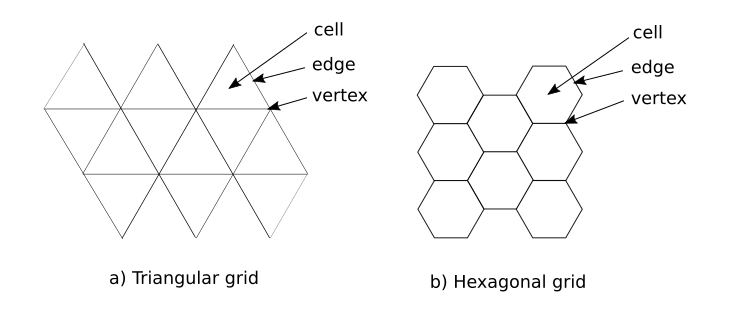
\includegraphics[width=.7\linewidth,natwidth=729,natheight=316]{hgrid.jpg}
  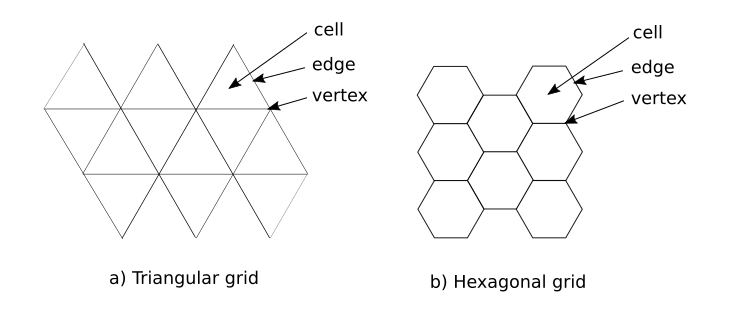
\includegraphics[width=.7\linewidth]{hgrid.jpg}
  \caption{Scope of variables inside the grids}
  \label{fig:grid}
\end{figure}

Larger grids are shown in \Cref{fig:triangulargrid} (and in \Cref{fig:hexagonalgrid}).
There are figures provided that illustrate the neighbourhood between data points and for different data localisation.

\paragraph{A triangular grid} consists of cells shaped as a triangle (\Cref{fig:grid-triangleempty}).
%It's structure is similar to the hexagonal grid.
Values can be located at the centres of the primal grid \Cref{fig:grid-trianglecenter}, and if we connect it, we would see the grid of triangles \Cref{fig:grid-trianglecenter_derived}.
If values are located at the edges (\Cref{fig:grid-triangleedges}) and they are connected with its neighbours, then the grid is given as in \Cref{fig:grid-triangleedges_derived}.
If the values are located at the vertices and they are connected with its neighbours, then the grid is given as in \Cref{fig:grid-trianglevertex}.

\paragraph{Hexagonal grid} consists of cells shaped as a flat topped hexagon (\Cref{fig:grid-hex-empty}).
Two ways can be used to map data to the grid: vertical or horizontal.
Values can be located at the centres of the primal grid (hexagons \Cref{fig:grid-hex-center}), and if we connect it, we would see a grid of triangles \Cref{fig:grid-hex-center_derived}.
If values are located at the edges (\Cref{fig:grid-hex-edges}) and edges are connected with those of the neighbours, then a grid as shown in \Cref{fig:grid-hex-edges_derived} emerges.
If the values are located at the vertices and vertices are connected with those of the neighbours, then a different grid emerges (see \Cref{fig:grid-hex-vertex}).


\subsection{Serialisation of Grids}
The abstractions of grids need to be serialised as data structures for the programming languages and for persisting them on storage systems.
In a programming language, regular grids can usually be addressed by n-dimensional arrays.
Thus, a 2D array can be used to store the data of a regular 2D longitude/latitude-based grid.

However, storing irregular grids is not so trivial.
For example, a 1D array can be used to hold the data, but then the index has to be determined.
Considering our 2D example, a mapping between the 2D coordinate and the 1D index has to be found.
One strategy to provide the mapping is space-filling curves.
These curves have the advantage that the indices to some extent preserve locality for points that are close together -- which can be beneficial, as often operations are conducted on neighbouring data (stencil operations, for example).
A Hilbert curve is an example of one possible enumeration of a multi-dimensional space.

{\bf The Hilbert curve} is a continuous space-filling curve, that helps to represent a grid as an n-dimensional array of values.
A 2D grid is shown in \Cref{fig:hilbert-test} to enable the visualisation of its behaviour.
In 2D, the fundamental element of the Hilbert curve is a square with one open side.
Every such square has two end-points, and each of these can be the entry-point or the exit-point.
%So, there are four possible varieties of the open side.
% ... varieties are entirely different mathematical objects; -P
So, there are four possible variations of the open side.
A first-order Hilbert curve consists of one fundamental element.
It is a 2x2 grid.
The second order Hilbert curve replaces this element by four (smaller) essential elements, which are linked together by three joins (4x4 grid).
Every next order repeats the process by replacing each element by four smaller elements and three joins (8x8 grid).
On the \Cref{fig:hilbert-test} the 5th level Hilbert curve is represented for the 256x256 data, that is mapped to a 32x32 grid.

The characteristics of a Hilbert curve can be extended to more than two dimensions.
The first step in the figure can be wrapped up in as many dimensions as is needed and the points/neighbours will always be saved.


\begin{figure}[!tbp]
 \centering
  \begin{subfigure}[b]{0.4\textwidth}
	 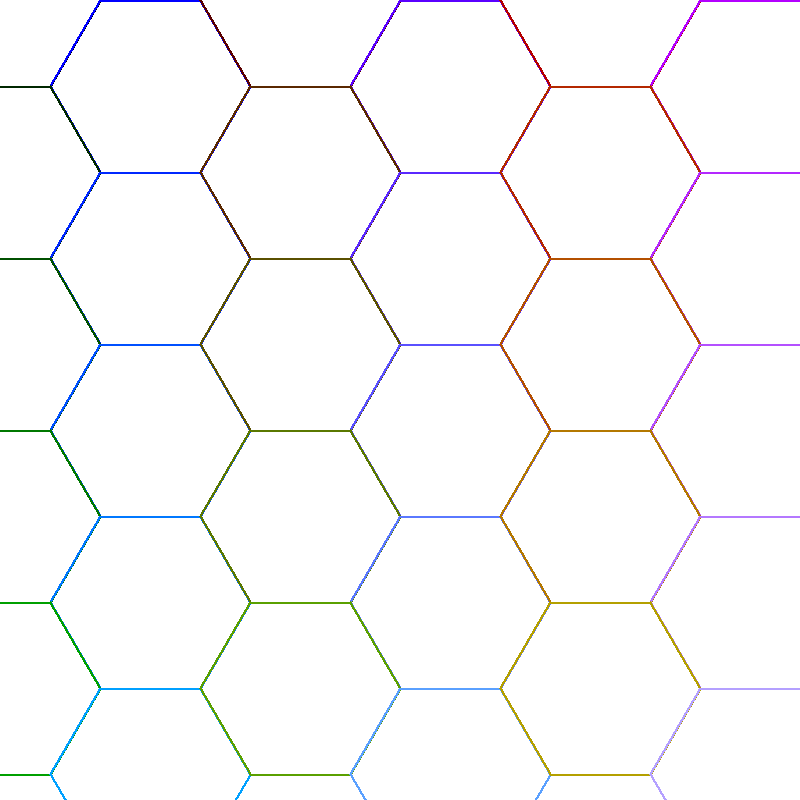
\includegraphics[width=\textwidth] {grid-hex-empty.png}
	 \caption{Empty hexagonal grid}
	 \label{fig:grid-hex-empty}
 \end{subfigure}
 \hfill
 \begin{subfigure}[b]{0.4\textwidth}
	 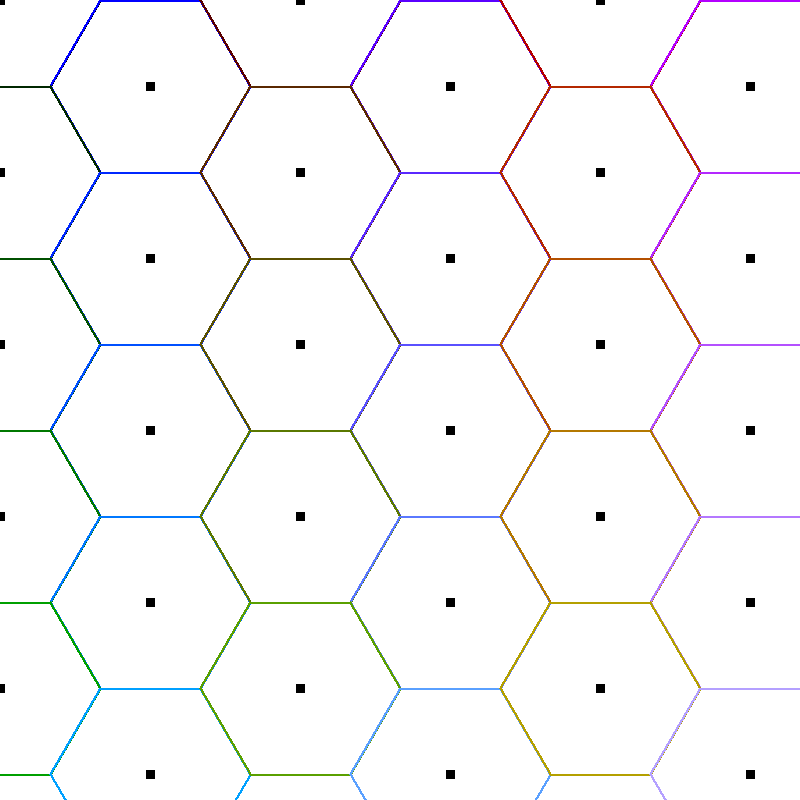
\includegraphics[width=\textwidth] {grid-hex-center.png}
	 \caption{Hexagonal grid with data at the cell centres.}
	 \label{fig:grid-hex-center}
 \end{subfigure}
 \hfill
 \begin{subfigure}[b]{0.4\textwidth}
	 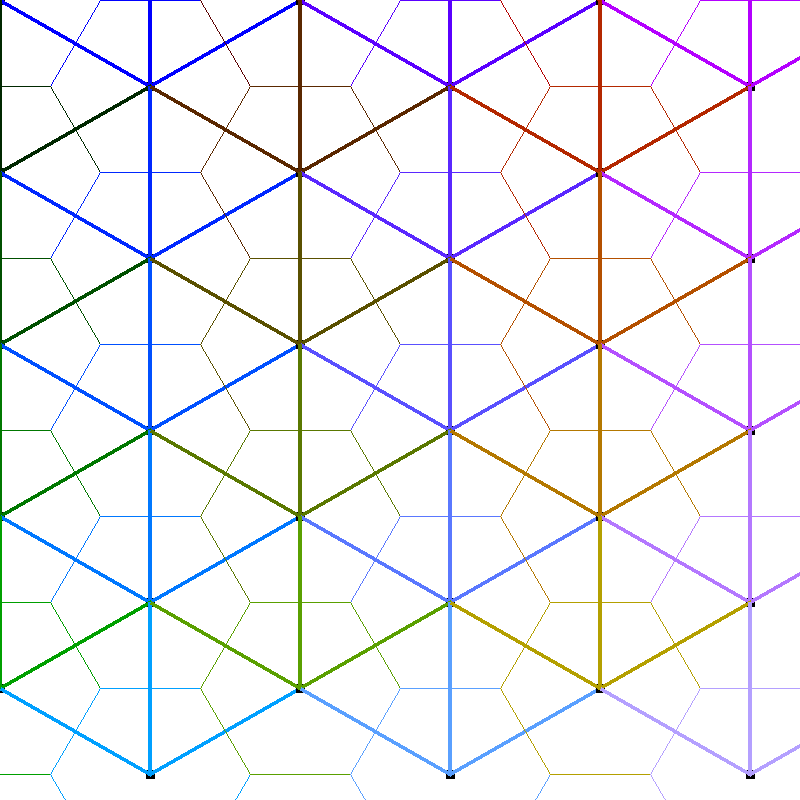
\includegraphics[width=\textwidth] {grid-hex-center_derived.png}
	 \caption{Hexagonal grid with data at the cell's centres, connected neighbours}
	 \label{fig:grid-hex-center_derived}
 \end{subfigure}
 \hfill
 \begin{subfigure}[b]{0.4\textwidth}
	 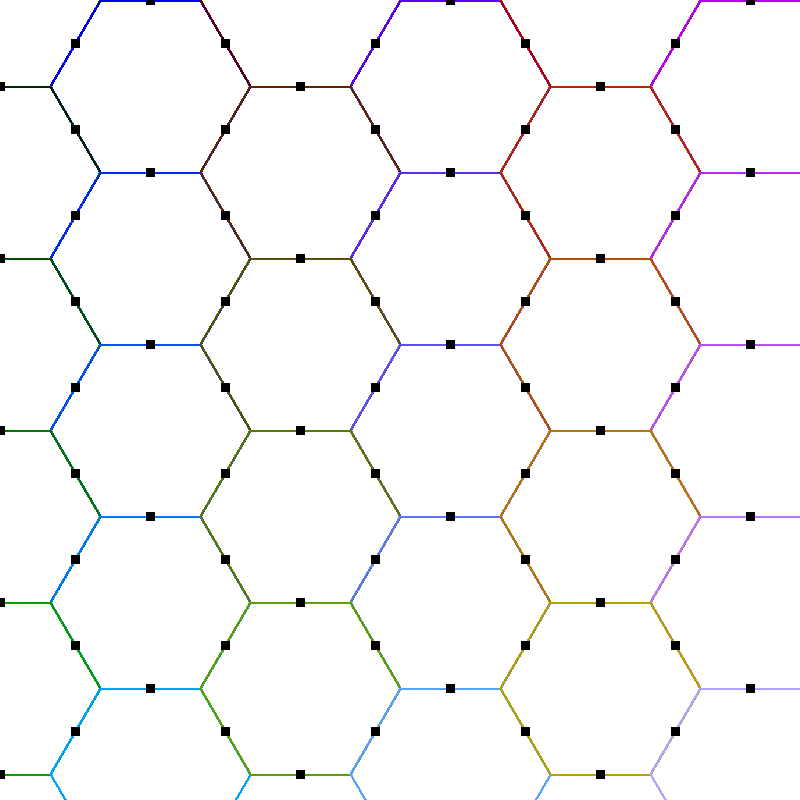
\includegraphics[width=\textwidth] {grid-hex-edges.png}
	 \caption{Hexagonal grid with data on the edges}
	 \label{fig:grid-hex-edges}
 \end{subfigure}
 \hfill
 \begin{subfigure}[b]{0.4\textwidth}
	 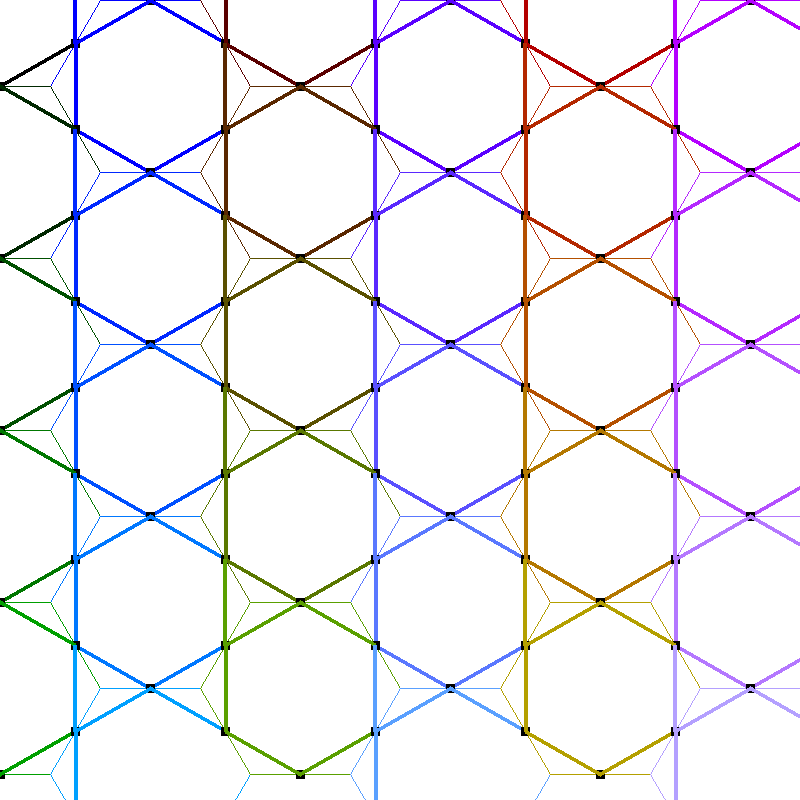
\includegraphics[width=\textwidth] {grid-hex-edges_derived.png}
	 \caption{Hexagonal grid with data on the edges, connected neighbours}
	 \label{fig:grid-hex-edges_derived}
 \end{subfigure}
 \hfill
 \begin{subfigure}[b]{0.4\textwidth}
	 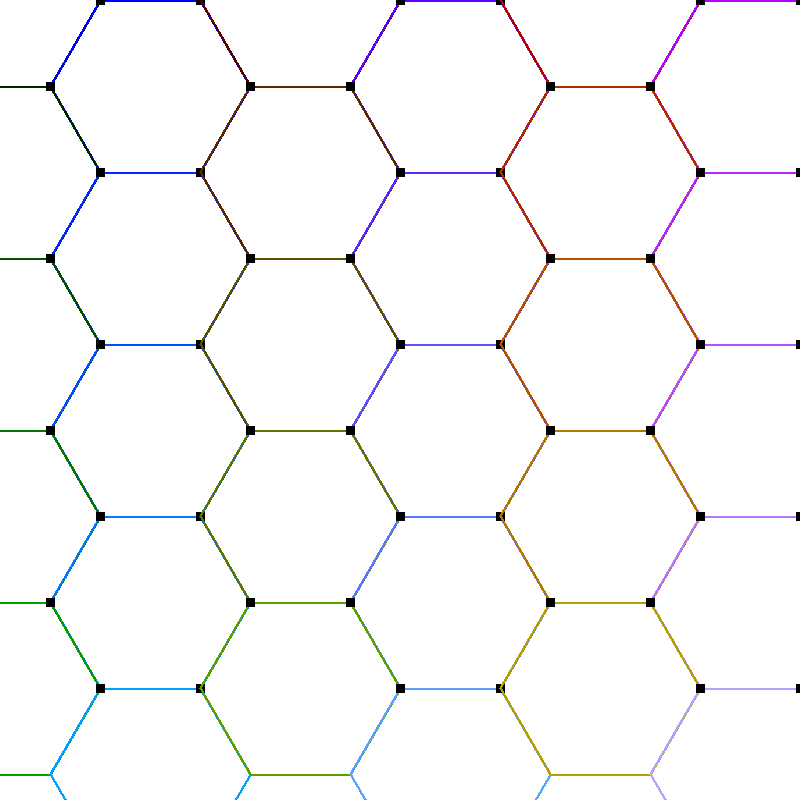
\includegraphics[width=\textwidth] {grid-hex-vertex.png}
	 \caption{Hexagonal grid with data at the vertices / connected neighbours}
	 \label{fig:grid-hex-vertex}
 \end{subfigure}

 \caption{Hexagonal grid}
 \label{fig:hexagonalgrid}
\end{figure}

\begin{figure}[!tbp]
 \centering
  \begin{subfigure}[b]{0.4\textwidth}
	 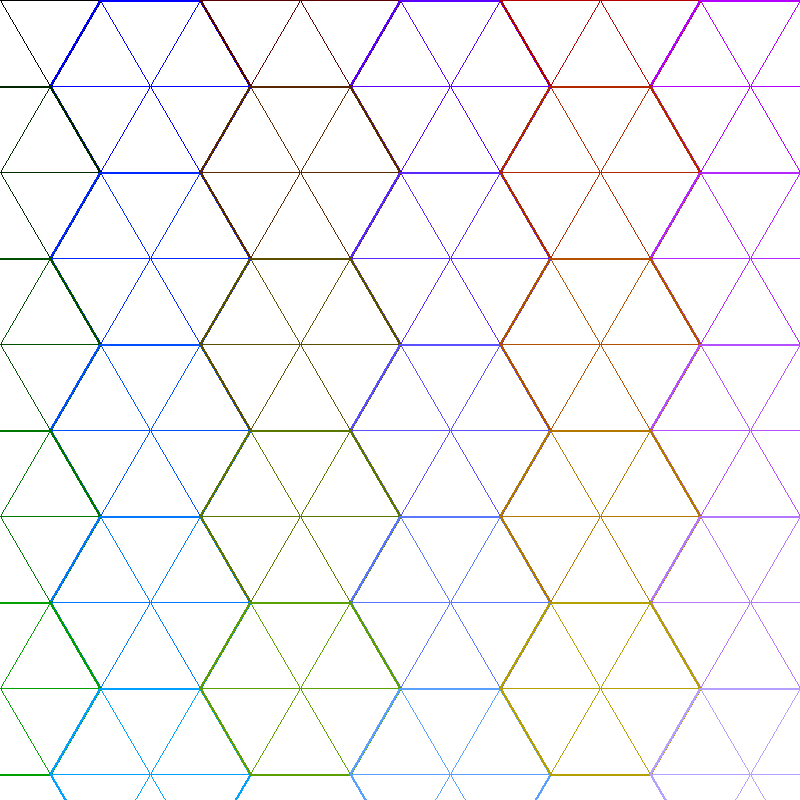
\includegraphics[width=\textwidth] {grid-triangleempty.png}
	 \caption{Empty triangular grid}
	 \label{fig:grid-triangleempty}
 \end{subfigure}
 \hfill
 \begin{subfigure}[b]{0.4\textwidth}
	 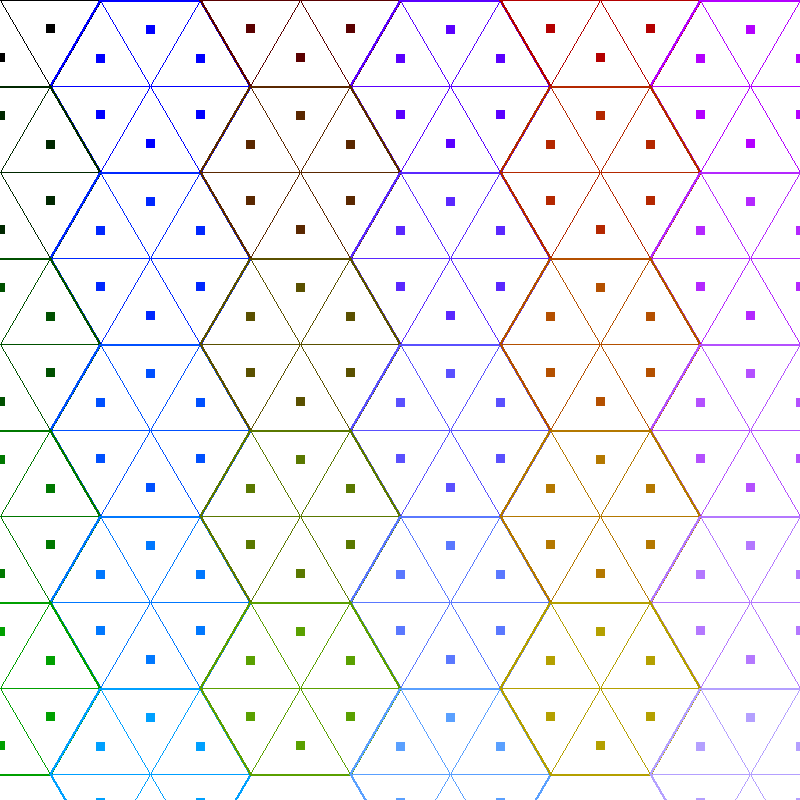
\includegraphics[width=\textwidth] {grid-trianglecenter.png}
	 \caption{Triangular grid with data at the cell centres}
	 \label{fig:grid-trianglecenter}
 \end{subfigure}
 \hfill
 \begin{subfigure}[b]{0.4\textwidth}
	 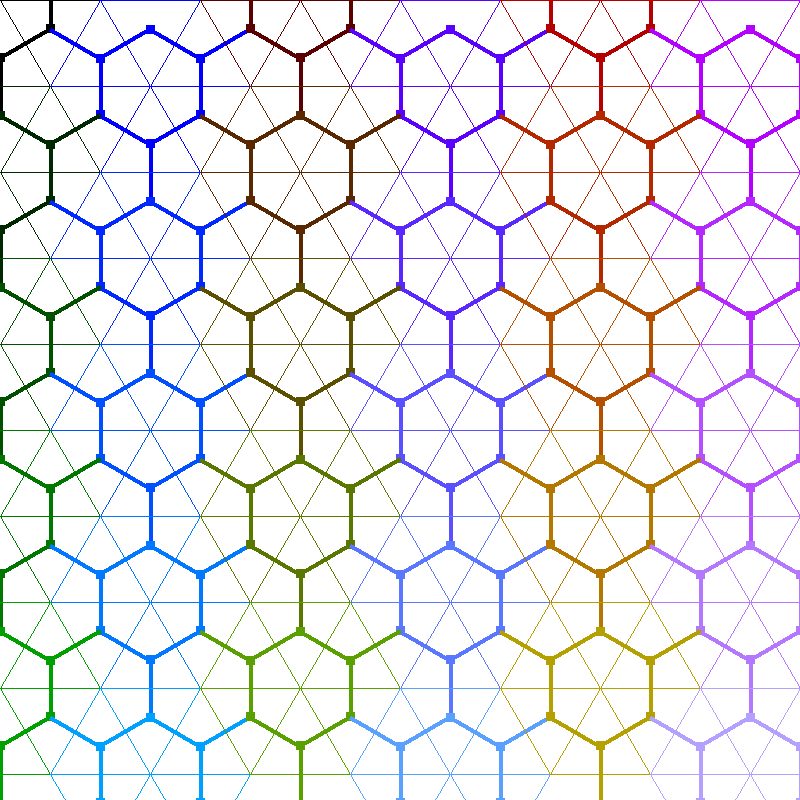
\includegraphics[width=\textwidth] {grid-trianglecenter_derived.png}
	 \caption{Triangular grid with data at the cell centres, connected neighbours}
	 \label{fig:grid-trianglecenter_derived}
 \end{subfigure}
 \hfill
 \begin{subfigure}[b]{0.4\textwidth}
	 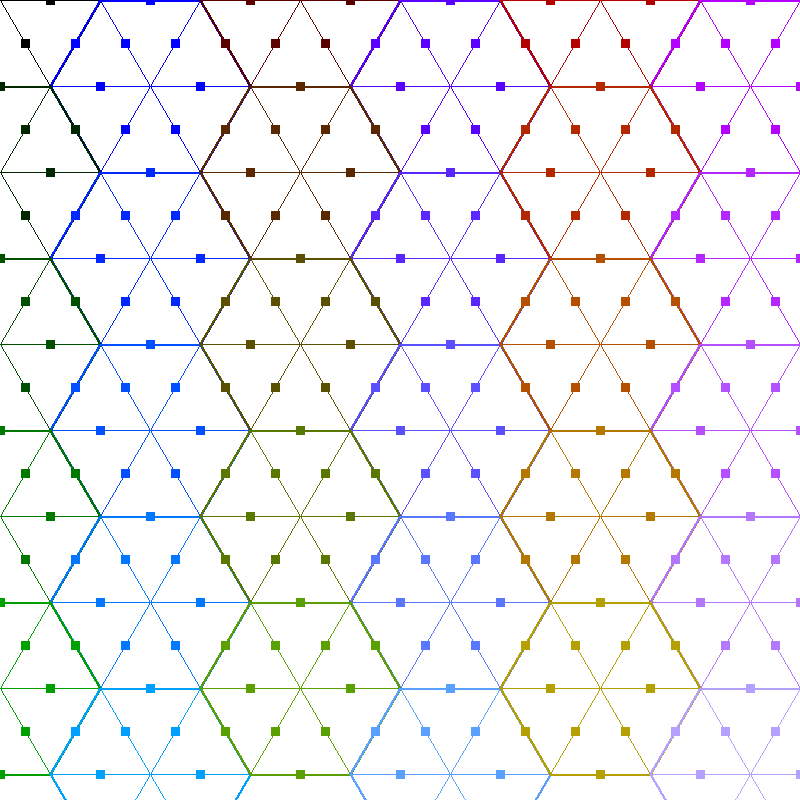
\includegraphics[width=\textwidth] {grid-triangleedges.png}
	 \caption{Triangular grid with data on the edges}
	 \label{fig:grid-triangleedges}
 \end{subfigure}
 \hfill
 \begin{subfigure}[b]{0.4\textwidth}
	 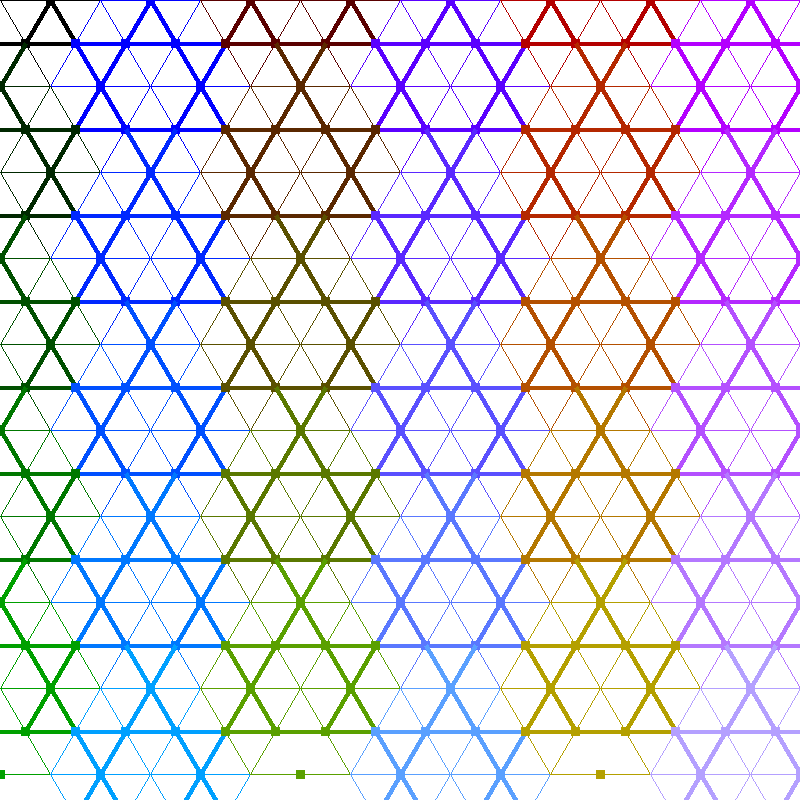
\includegraphics[width=\textwidth] {grid-triangleedges_derived.png}
	 \caption{Triangular grid with data on the edges, connected neighbours}
	 \label{fig:grid-triangleedges_derived}
 \end{subfigure}
 \hfill
 \begin{subfigure}[b]{0.4\textwidth}
	 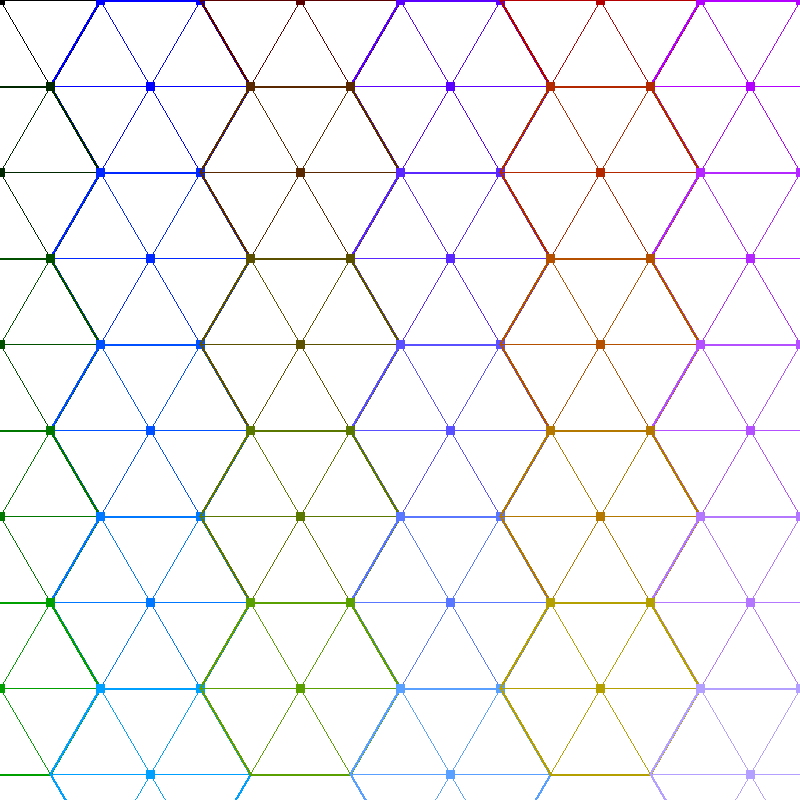
\includegraphics[width=\textwidth] {grid-trianglevertex.png}
	 \caption{Triangular grid with data on the vertices / connected neighbours}
	 \label{fig:grid-trianglevertex}
 \end{subfigure}
 \caption{Triangular grid}
 \label{fig:triangulargrid}
\end{figure}

%\begin{figure}[!tbp]
% \centering
% \adjincludegraphics[trim={0 {.875\height} {.875\width} 0},clip] %{test.png}
% \caption{Hilbert space-filling curve}
% \label{fig:hilbert-test}
%\end{figure}

\begin{figure}[!tbp]
 \centering
 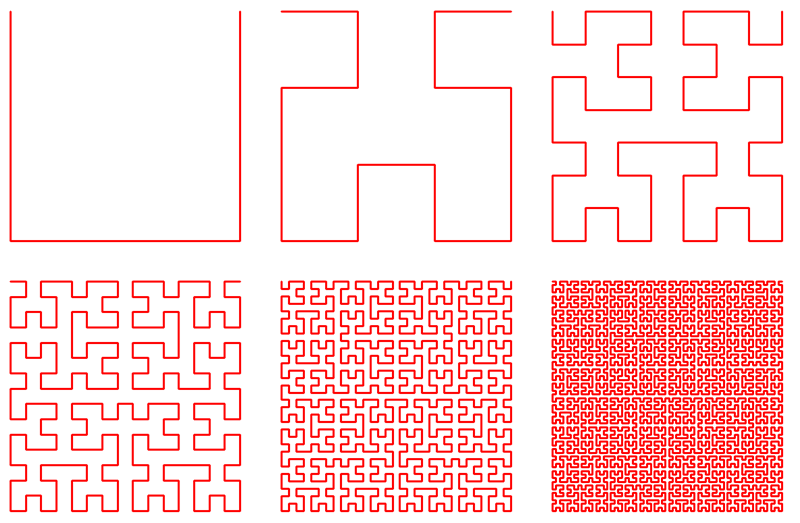
\includegraphics[width=\textwidth] {pattern.png}
 \caption{Hilbert space-filling curve}
 \label{fig:hilbert-test}
\end{figure}

\paragraph{Considerations when serialising to storage systems}

%\todo{@Bryan/Julian: This is where we link the previous material to the storage system
%futures and hence relevance to architecture, but it needs to be more explicit.}

When serialising a data structure to a storage system, in essence, this can be done similarly as in main memory.
The address space exported by the file API of a traditional file system considers the file to be an array of bytes starting from 0 which is quite similar to the 1D structure from main memory.
However, a general purpose language (GPL) uses variable names to point to the data in this 1D address space.
A GPL offers means to access even multi-dimensional data easily.
The user/programmer does not need to know the specific addresses in memory; addresses are calculated within the execution environment or code of the application.
The main concern here is consecutive or stride access through the array; if the programmer wishes the application to loop through a given dimension of the array, memory locations would be addressed which may not be close to each other in memory, thus leading to cache misses and hence more unsatisfactory performance.
The generalisation is the stride, which specifies steps through the different dimensions of the array (e.g. incrementing both dimensions of a 2D array, thus walking along the ``diagonal'').
Another particular case is where the programmer needs to process the whole array, which would be done most efficiently by stepping through all the memory locations incrementally\footnote{Assuming the entire array is stored in contiguous memory, as it is in these simple examples.},
whereas looping over the dimensions and incrementing them one at a time requires more calculations and may lead to inefficient memory access with cache misses if not done correctly\footnote{Fortran historically stores 2D arrays in column-major order, whereas C and most other languages used in science store data in row-major order.}.

% problematic, as they = ?
%as they are implicitly known by the code and relatively defined by the execution environment of the application in the form of stack and heap.

\medskip

When storing data from memory directly on persistent media, the source code is necessary to understand this data.
Similarly, the interpretation of the bytes in the data must be the same when reading it back. Thus, the byte order and size of the data types of the machine reading the data must be identical to those of the device that wrote it.  Floating point numbers must be encoded in the same byte formats.
Since this is not always given, it threatens the longevity of our precious data, by hindering the portability and reusability of the data.

Therefore, portable data formats have been developed that allow serialising and deserialising data regardless of the machine's architecture.
To allow correct interpretation of a byte array, the library implementing the file format must know the data type that the bytes represent.
This information must be stored beside the actual bytes representing the data to allow later reading and interpretation.
From the user perspective, it is useful also to store further metadata describing the data (for instance, a name and a description of the contained information).
This practice eases not only debugging but also allows other applications to read and process data.
File formats that contain this semantical and structural metadata are called \textbf{self-describing file formats}.

Developers using a self-describing file format have to use an API to define the metadata.
Such a format may support arbitrary complex data types, which implies that some data description framework must be part of the API for the file format.
See \Cref{sec: data-formats} for more information about data description frameworks.


\section{File formats}
\label{sec: background/file formats}

%\todo{This section is written from a ``simulation'' only perspective. Need to consider read/write separately, and different aspects of aspects of parallelisation. What about MPI targeted write to OSDS? What about SAFE?}

Generally, parallel scientific applications are designed in such a way they can solve complicated problems faster when running on a large number of compute nodes.
The speed-up is achieved by splitting a global problem into small pieces and distributing them over multiple compute nodes; this is called domain decomposition.
After each node has computed a local solution, they can be aggregated to one global solution.
This approach can decrease time-to-solution considerably.

I/O makes this picture more complicated, especially when data is stored in one single file and is accessed by several processes simultaneously.
In this case, problems can occur, when several processes access the same file region, e.g., two processes can overwrite the data of each other, or inconsistencies can occur when one process reads, while another writes.
Portability is another issue: When transferring data from one platform to another, the contained information should still be accessible and identical.
The purpose of I/O libraries is to hide the complexity from scientists, allowing them to concentrate on their research.



\begin{table}
  \centering
  \begin{tabular}{l|l|l|l}
    Name      & Full Name                   & Version & Developer \\
    \hline
    GRIB1     & GRIdded Binary             & 1       & World Meteorological Organisation\\
    GRIB2     & GRIdded Binary             & 2       & World Meteorological Organisation\\
    NetCDF3   & Network Common Data Form   & 3.x     & Unidata (UCAR/NCAR)\\
    NetCDF4   & Network Common Data Format & 4.x     & Unidata (UCAR/NCAR\\
    HDF4      & Hierarchical Data Format   & 4.x     & NCSA/NASA\\
    HDF4-EOS2 & HDF4-Earth Observing System & 2       & \\
    HDF5      & Hierarchical Data Format   & 5.x     & NCSA/NASA\\
    HDF5-EOS5 & HDF5-Earth Observing System & 5       & \\
\end{tabular}
\caption{Parallel data formats}
\label{tab:fformats}
\end{table}


Some standard file formats are listed in the \Cref{tab:fformats}.
All of these formats are portable (machine independent) and self-describing.
Self-describing means that files can be examined and read by the appropriate software without the knowledge about the structural details of the data.
The files may include additional information about the data, called ``metadata''.
Often, it is textual information about each variable's contents and units (e.g., ``humidity'' and ``g/kg'') or numerical information describing the coordinates (e.g., time, level, latitude, longitude) that apply to the variables in the file.

GRIB is a record format, NetCDF/HDF/HDF-EOS formats are file formats.
%It is the difference.
In contrast to record format, file formats are bound to format specific rules.
For example, all variable names in NetCDF must be unique.
In HDF, although, variables with the same name are allowed, they must have different paths.
No such rules exist for GRIB.
It is just a collection of records (data sets), which can be appended to the file in any order.

GRIB-1 record (aka, ``message'') contains information about two horizontal dimensions (e.g., latitude and longitude) for one time and one level.
GRIB-2 allows each record to contain multiple grids and levels for each time.
However, no rules are dictating the order of the collection of GRIB records (e.g., records can be in random chronological order).

%Not HPC:
Finally, a file format without parallel I/O support, but still worth to mention, is CSV (comma-separated values).
It is distinctive due to its simplicity, broad acceptance and support by a wide range of applications.
The data is stored as plain text in a table.
Each line of the file is a data record.
Each record consists of one or more fields, that are separated by commas (hence the name).
The CSV file format is not standardised.
Many implementations support additional features, e.g., other separators and column names.



\subsection{NetCDF4}

NetCDF4 with Climate Forecast (CF) metadata has evolved to be the de facto standard format for convenient data access for climate scientists.

It provides a set of features to enable convenient data access. For example, metadata can be used to assign names to variables, set units of measure, label dimensions, and provide other useful information.
Portability allows data movement between different and possibly incompatible platforms, simplifying the exchange of data and facilitating communication between scientists.
The ability to grow and shrink data sets, add new data sets and access small data ranges within data sets expedites the handling of data.
%HPC: Sharable
Shared file access allows keeping the data in the same file, but
unfortunately, it conflicts with performance and efficient usage of state-of-art HPC.
Simultaneous access by several processes causes synchronisation overhead which slows down I/O performance (
the synchronisation is necessary to keep the data consistent).
%Performance: Compression, Chunking

% Relation between HPC imbalance and compression
The rapid development of computational power and storage capacity and slow development of network bandwidth and I/O performance in the last years resulted in imbalanced HPC systems.
Applications use the increased computational power to create more data.
More data, in turn, requires more costly storage space, higher network bandwidth and sufficient I/O performance on storage nodes.
But due to imbalance, the network and I/O performance are the main bottlenecks.
They can be offset to some extent by using a part of the computational power for compression, adding a little extra latency for the transformation while significantly reducing the amount of data that needs to be transmitted or stored.
% Transition to NetCDF4 and HDF5
However, before considering a compression method for HPC, it is a good idea to take a look at the realisation of parallel I/O in modern scientific applications.
Many of them use the NetCDF4 file format, which, in turn, uses HDF5 under the hood.

\subsection{Typical NetCDF Data Mapping}
\label{sec:netcdfDataMapping}
\Cref{lst:NetCDF-data} gives an example for scientific metadata stored in a NetCDF file.
Firstly, between Line 1 and 4, a few dimensions of the multi-dimensional data are defined.
Here there are longitude, latitude with a fixed size and time with a variable size that allows being extended (appending from a model).
Then different variables are defined on one or multiple of the dimensions.
The longitude variable provides a measure in “degrees east” and is indexed with the longitude dimension; in that case, the variable longitude is a 1D array that contains values for an index between 0-479.
It is allowed to define attributes on variables. This scientific metadata can define the semantics of the data and provide information about the data provenance.
In our example, the unit for longitude is defined in Line\,7.
Multi-dimensional variables such as \texttt{sund} (Line 17) are defined on a 2D array of values for the longitude and latitude over various timesteps.
The numeric values contain a scale factor and offset that has to be applied when accessing the data; since, here, the data is stored as short values, it should be converted to floating point data in the application.
The \texttt{\_FillValue} indicates a default value for missing data points.

Finally, global attributes such as indicated in Line\,33\, describe that this file is written with the NetCDF-CF schema and its history describes how the data has been derived/extracted from original data.

\begin{tcbcode}[label={lst:NetCDF-data}]{Example NetCDF metadata}
\begin{lstlisting}
dimensions:
	longitude = 480 ;
	latitude = 241 ;
	time = UNLIMITED ; // (1096 currently)
variables:
	float longitude(longitude) ;
		longitude:units = "degrees_east" ;
		longitude:long_name = "longitude" ;
	float latitude(latitude) ;
		latitude:units = "degrees_north" ;
		latitude:long_name = "latitude" ;
	int time(time) ;
		time:units = "hours since 1900-01-01 00:00:0.0" ;
		time:long_name = "time" ;
		time:calendar = "Gregorian" ;

	short t2m(time, latitude, longitude) ;
		t2m:scale_factor = 0.00203513170666401 ;
		t2m:add_offset = 257.975148205631 ;
		t2m:_FillValue = -32767s ;
		t2m:missing_value = -32767s ;
		t2m:units = "K" ;
		t2m:long_name = "2 metre temperature" ;
	short sund(time, latitude, longitude) ;
		sund:scale_factor = 0.659209863732776 ;
		sund:add_offset = 21599.6703950681 ;
		sund:_FillValue = -32767s ;
		sund:missing_value = -32767s ;
		sund:units = "s" ;
		sund:long_name = "Sunshine duration" ;

// global attributes:
		:Conventions = "CF-1.0" ;
		:history = "2015-06-03 08:02:17 GMT by grib_to_netcdf-1.13.1: grib_to_netcdf /data/data04/scratch/netcdf-atls14-a562cefde8a29a7288fa0b8b7f9413f7-lFD4z9.target -o /data/data04/scratch/netcdf-atls14-a562cefde8a29a7288fa0b8b7f9413f7-CyGl1B.nc -utime" ;
}
\end{lstlisting}
\end{tcbcode}

% \todo{(BNL) A proper semantic discussion to allow us to introduce "cross-file " aggregation would introduce the CF standard here and then discuss the CF aggregation rules and how they need to be supported in the architecture. Agreed !}

%\subsection{SAFE}
% \todo{BNL4BNL: Need to introduce SAFE and describe how much of it is supportable
% within any ESD architecture - leading to a specific requirement in the logical
% view.}
